\documentclass[12pt, letterpaper]{article}

\usepackage[utf8]{inputenc}
\usepackage{booktabs}
\usepackage[table,xcdraw]{xcolor}
\usepackage{hyperref}
\hypersetup{
    colorlinks=true, %set true if you want colored links
    linktoc=all,     %set to all if you want both sections and subsections linked
    linkcolor=black,  %choose some color if you want links to stand out
}
\usepackage{graphicx}
\graphicspath{{./images/}}
\usepackage{float}

\usepackage[none]{hyphenat}

\tolerance=1
\emergencystretch=\maxdimen
\hyphenpenalty=10000
\hbadness=10000

\title{Sistema Gestione ZTL}
\author{Riccardo Maria Pesce}
\date{Anno Accademico 2019-2020}

\renewcommand{\contentsname}{Contenuti}

\begin{document}

\begin{titlepage}

\maketitle

\begin{abstract}

\noindent
In questo documento eseguiremo l'analisi orientata
agli oggetti ed in seguito la progettazione.
Inizieremo stilando quelli che saranno i requisiti 
ed i casi d'uso implementati, illustreremo il modello
di dominio ed i diagrammi di sequenza di sistema.

\end{abstract}
\end{titlepage}

\tableofcontents{}

\pagebreak

\section{Piano di analisi e progettazione}
Durante la prima iterazione, abbiamo deciso di 
analizzare ed implementare i sequenti requisiti 
e casi d'uso:
\begin{itemize}
    \item Lo scenario principale di successo del 
    caso d'uso UC1 (Registra Ingresso), solo per 
    utente residente
    \item Lo scenario principale di successo del 
    caso d'uso UC2 (Registra Uscita), solo per 
    utente residente
\end{itemize}
Si è deciso di impletare quanto sopra per poter 
verificare (attraverso un futuro meeting di proof-
of-concepts) che i requisiti base del sistema si 
siano compresi.
Inoltre, vogliamo dare precedenza ai residenti nello 
sviluppo, in modo tale che, una volta che tutta
l'infrastruttura elettronica sarà pronta, possiamo
fornire un sistema funzionante limitatamente a
loro.
\linebreak

\noindent
Riportiamo qui i casi d'uso di cui sopra. Per 
un maggior dettaglio, consultare il documento di 
ideazione (Ideazione.pdf), dove sono gia espressi
dettagliatamente. I casi d'uso qui riportati 
includono solo ciò che è di interesse per questa 
iterazione. I casi d'uso sono stati leggermente 
ridefiniti in quanto non era molto chiaro il 
meccanismo di ingresso/uscita.

\subsection{Caso d'uso UC1 - Registra Ingresso}

\begin{itemize}
\item \textbf{UC1:} Registra Ingresso
\item \textbf{Portata:} Sistema Gestion ZTL
\item \textbf{Livello:} Obiettivo utente
\item \textbf{Pre-condizioni:} Nessuna
\item \textbf{Garanzie di successo (Post-condizioni):} L'utente identificato entra nella ZTL

\item \textbf{Scenario principale di successo}
\begin{itemize}
    \item L'utente, avvicinatosi al varco, innesta il sistema attraverso l'invio, da parte del telepass, di un codice identificativo
    \item Il valico lo lascia passare inviando come 
    risposta il codice identificativo stesso 
\end{itemize}

\item \textbf{Requisiti speciali:} Bassa latenza
\item \textbf{Frequenza:} Ogni qualvolta un utente si presenta al varco
\end{itemize}

\subsection{Caso d'uso UC2 - Registra Uscita}
\begin{itemize}
\item \textbf{UC2:} Registra Uscita
\item \textbf{Portata:} Sistema Gestion ZTL
\item \textbf{Livello:} Obiettivo utente
\item \textbf{Pre-condizioni:} L'utente si trova all'interno della zona a traffico limitato
\item \textbf{Garanzie di successo (Post-condizioni):} L'utente esce dalla zona a traffico limitato
\item \textbf{Scenario principale di successo}
\begin{itemize}
    \item L'utente, avvicinatosi al varco d'uscita, attiva il sistema attraverso l'invio, da parte del telepass, di un codice identificativo.
    \item Il valico lo lascia passare inviando come 
    risposta il codice identificativo stesso    
\end{itemize}   

\item \textbf{Requisiti speciali:} Bassa latenza
\item \textbf{Frequenza:} Ogni qualvolta un utente si presenta al varco
\end{itemize}

\section{Modello di Dominio}
Osservando i casi d'uso, si osservano le seguenti
classi concettuali:
\begin{itemize}
    \item \textbf{Residente:} l'utente (inteso
    come veicolo, come precisato gia) che possiede
    casa all'interno della zona a traffico limitato
    e che gode di accesso illimitato senza vincoli
    Esso è univocamente identificato dal codice ID,
    anche se la telecamera CTV può registrare la 
    targa.
    \item \textbf{Terminale:} dispositivo ai varchi 
    della zona a traffico limitato
    \item \textbf{Accesso:} istanza d'accesso alla 
    zona a traffico limitato
    \item \textbf{Uscita:} istanza d'uscita dalla 
    zona a traffico limitato
    \item \textbf{SistemaGestioneZTL:} il software
    che gira sul server centrale e che coordina
    le varie attività
\end{itemize}

\subsection{Modello di Dominio UC1}
\begin{figure}[H]
    \centering
    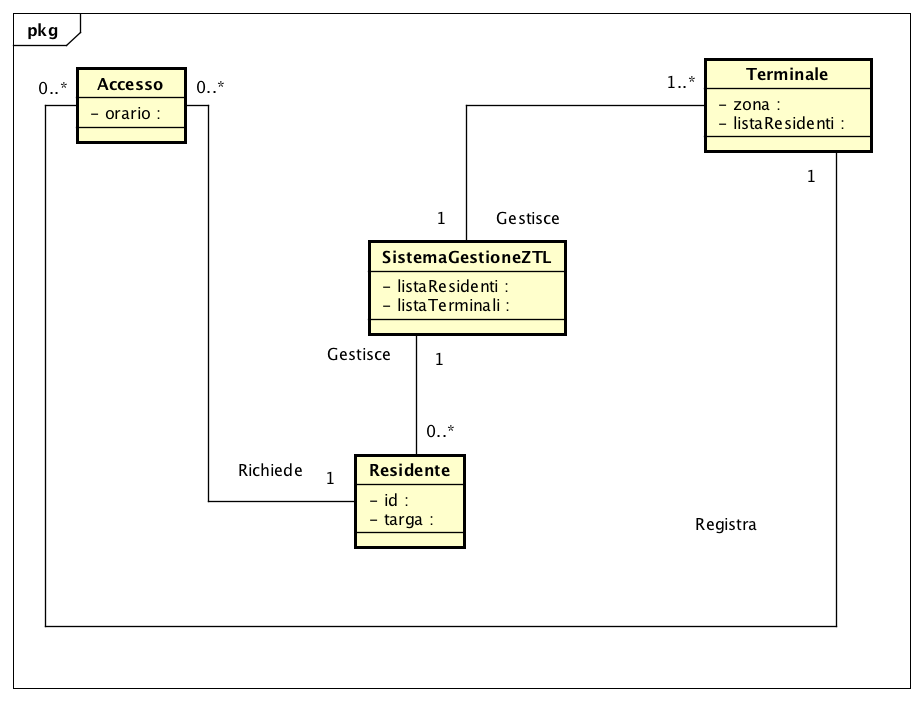
\includegraphics[scale=0.50]{I1-UC1-DM}
    \label{fig:mesh1}
\end{figure}

\subsection{Modello di Dominio UC2}
\begin{figure}[H]
    \centering
    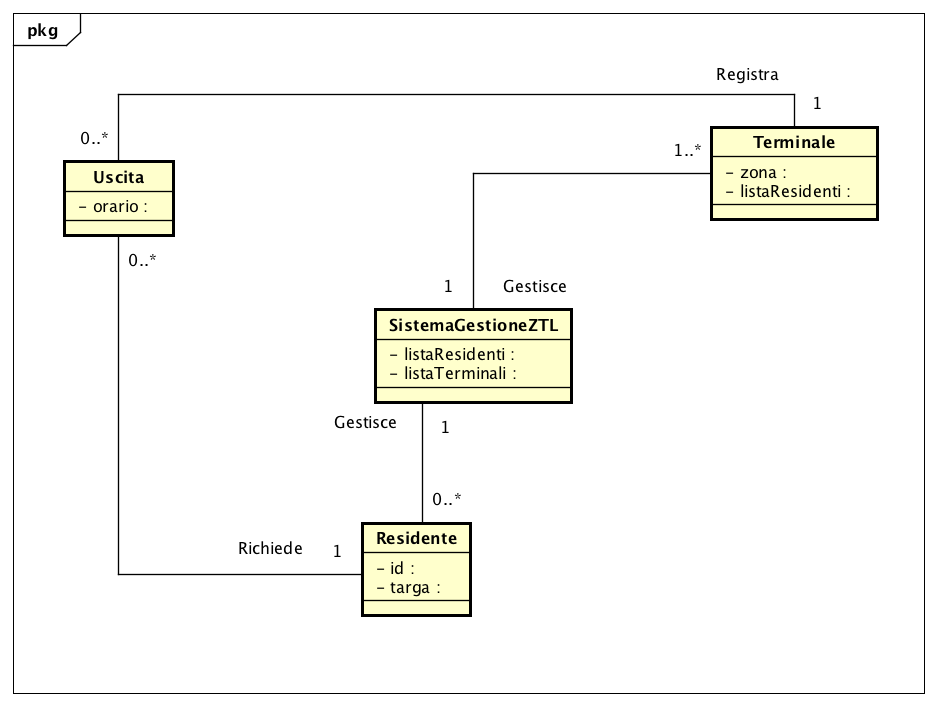
\includegraphics[scale=0.50]{I1-UC2-DM}
    \label{fig:mesh1}
\end{figure}

\section{Diagrammi di Sequenza di Sistema}
I diagrammi di sequenza di sistema mostrano
lo scambio di messaggi tra attori esterni 
e sistema. 

\subsection{Diagrammi di Sequenza di Sistema UC1}
\begin{figure}[H]
    \centering
    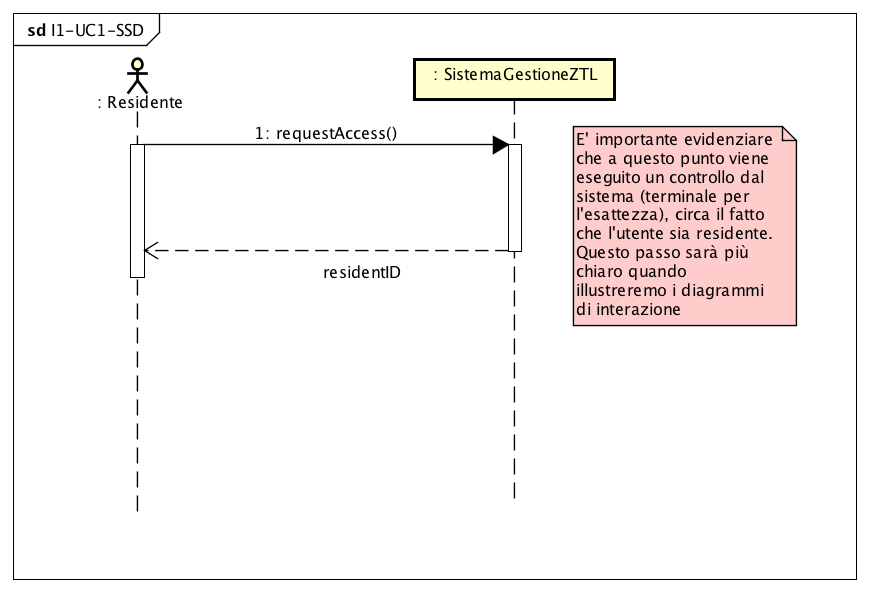
\includegraphics[scale=0.50]{I1-UC1-SSD}
    \label{fig:mesh1}
\end{figure}

\subsection{Diagrammi di Sequenza di Sistema UC2}
\begin{figure}[H]
    \centering
    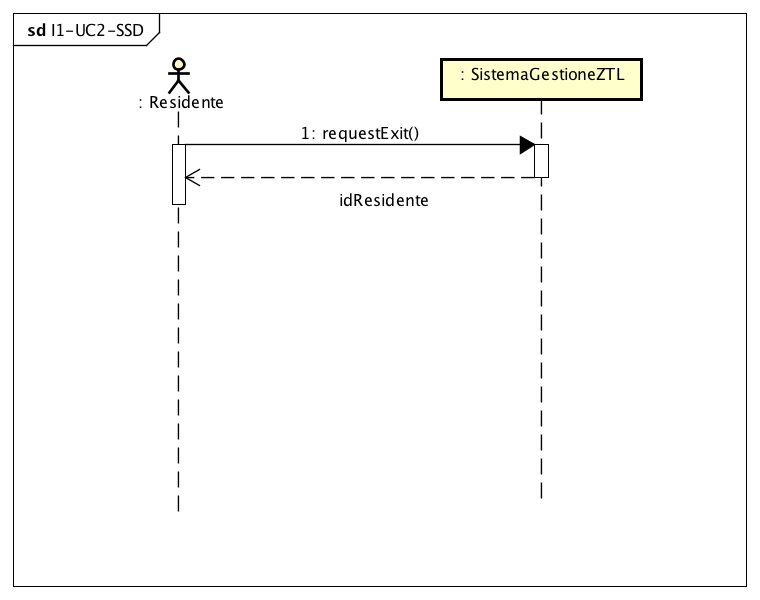
\includegraphics[scale=0.50]{I1-UC2-SSD}
    \label{fig:mesh1}
\end{figure}

\section{Contratti delle operazioni}
Si sono individuati le seguenti operazioni 
per tale iterazione:
\subsection{CO1 - Operazione: \texttt{richiediAccesso(id : int)}}
\begin{itemize}
    \item \textbf{Riferimenti:} Caso d'uso UC1
    \item \textbf{Pre-condizioni:} un residente si
    presenta al varco d'accesso
    \item \textbf{Post-condizioni:} il residente 
    accede alla zona a traffico limitato
\end{itemize}

\subsection{CO2 - Operazione: \texttt{richiediUscita(id : int)}}
\begin{itemize}
    \item \textbf{Riferimenti:} Caso d'uso UC2
    \item \textbf{Pre-condizioni:} un residente si
    presenta al varco d'uscita
    \item \textbf{Post-condizioni:} il residente 
    esce dalla zona a traffico limitato
\end{itemize}

\noindent
Nelle prossime iterazioni, quando includeremo
le funzionalità per utenti carico-scarico,
tali contratti subiranno alcune modifiche.

\section{Diagramma delle Interazioni}
Le interazioni fra le varie componenti del sistema, 
per entrambe le iterazioni, sono alquanto triviali:
ogni terminale controlla la lista di residenti, e, 
trovato l'ID del residente ricercato, lo restituisce.
Mostreremo solo gli scenari di successo: in caso 
l'id non fosse presente, verrà stampato a video,
e nelle successive iterazioni ci occuperemo meglio
dei casi alternativi.

\subsection{Diagramma delle Interazioni UC1}
\begin{figure}[H]
    \centering
    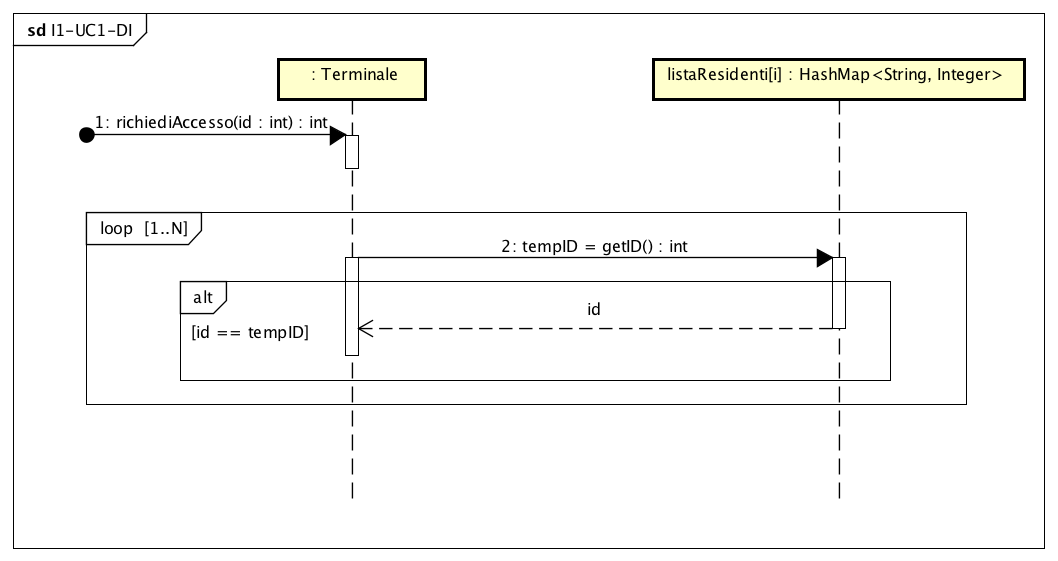
\includegraphics[scale=0.45]{I1-UC1-DI}
    \label{fig:mesh1}
\end{figure}

\subsection{Diagramma delle Interazioni UC2}
\begin{figure}[H]
    \centering
    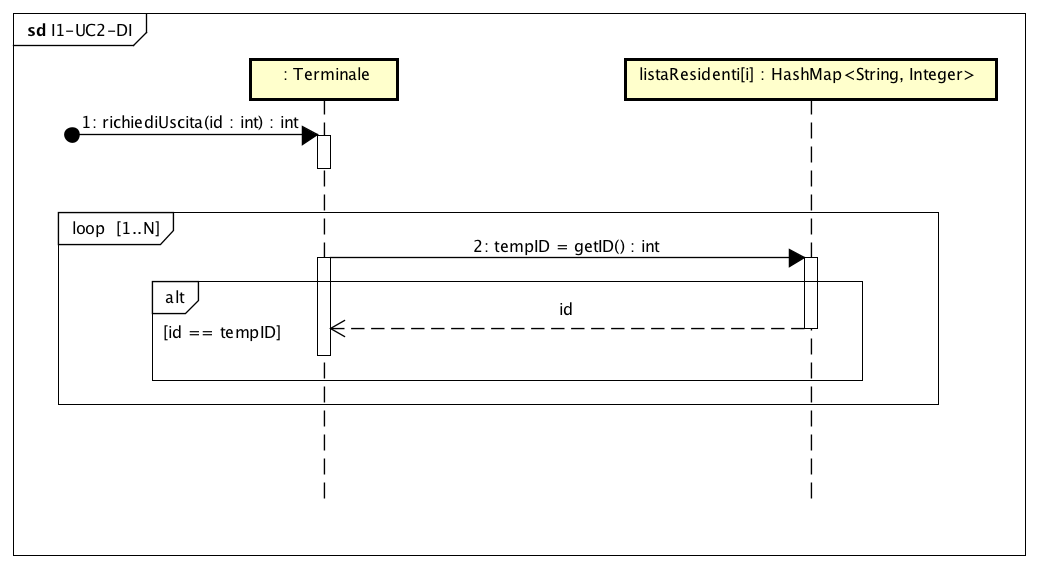
\includegraphics[scale=0.45]{I1-UC2-DI}
    \label{fig:mesh1}
\end{figure}

\section{Diagramma delle Classi Progettuali}
Nel diagramma delle classi progettuali, non vogliamo 
aggiungere la classe \emph{Utente}, usata solo a fini
simulativi e che quindi non farà parte del prodotto
finale consegnato.
\begin{figure}[H]
    \centering
    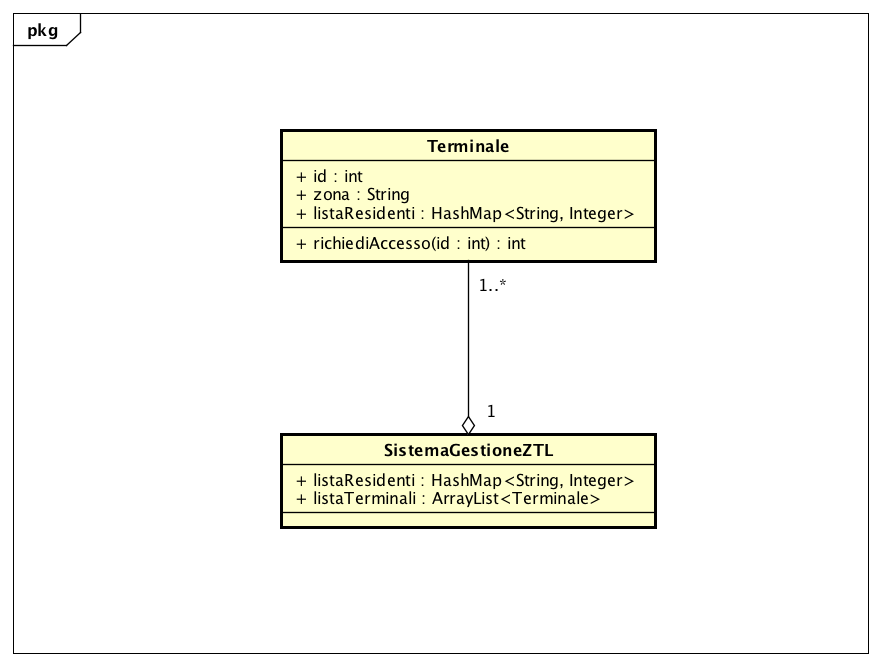
\includegraphics[scale=0.45]{DCD}
    \label{fig:mesh1}
\end{figure}


\section{Motivazioni progettuali}
\subsection{Classi Test-Driver}
Per realizzare i test strutturali, viene creata una
classe software che interagisce con il sistema come 
farebbe un utente nella vita reale. 
Tale classe sarà appunto la classe \emph{Utente} e conterrà
le informazioni Utente (id e targa) ed alcuni 
metodi per interagire con i terminali ed il 
sistema centrale. Tale classe non è inclusa 
nella progettazione dei diagrammi in quanto 
non fa parte del sistema.

\subsection{Sistema Centrale e Pattern \emph{Singleton}}
Il sistema centrale necessita di un meccanismo che 
garantisca la sua unicità. Utilizzeremo pertanto
il Pattern \emph{Singleton}.

\section{Casi di Test}

\subsection{Test Unitari dei casi d'uso UC1 ed UC2}
Ci assicureremo che i metodi \texttt{richiediAccesso()} e 
\texttt{richiediUscita()} ritornino l'ID se l'utene è 
residente, \emph{-1} in caso contrario. 
Questo ci permette di constatare che il dispositivo 
invii il codice identificativo esatto per ogni 
transito regolare (limitato, in questa iterazione,
solo ai residenti).

\end{document}